\documentclass[twocolumn,8pt]{article}

\topmargin    -10pt % Might need to be set to 0pt 
                      % for some installations

\textheight    610pt
\columnsep      24pt


\title{Real-Time HDR Image Based Lighting}


\author{Jo\~{a}o Pedro Jorge\thanks{joajo939@student.liu.se} \and Willem Frishert\thanks{wilfr265@student.liu.se}}
\date{27-05-2007}

\usepackage{subfigure}
\usepackage[pdftex]{graphicx}

\begin{document}
\small

\maketitle
\begin{abstract}
This report presents the work done on the final project for the course of Image Based Rendering. A real-time application has been implemented with the purpose of demonstrating the capabilities of nowadays GPU's power within the scope of Image Based Rendering and Lighting. The built application has a full High Dynamic Range (HDR) pipeline and it deals with issues like tone mapping, automatic scene exposure, vignette effect and blooming (to increase the high dynamic effect). Furthermore, some materials were used to demonstrate the potentiality of Image Based Lighting.
\end{abstract}
\\ \\
{\bf Keywords:}
Image Based Lighting, HDR, Tone Mapping, Real-Time.

\section{Introduction}
HDR images, in comparison to normal digital imaging techniques, contain a high dynamic range of intensities. Given these high range intensities, HDR images are able to convey a more realistic idea of the scene (through tone mapping techniques, given the screen restrictions). HDR images can be used as light sources for rendering - a technique referred to as Image Based Lighting (IBL). The goal of this project is to performed HDR IBL at real-time using hardware accelerated graphics.

To gain an understanding on how to construct an HDR pipeline, some ideas were taken from real-time HDR IBL implementations that currently exist. Example implementations are Masaki Kawase's rthdribl and ATI's real-time version of Debevec's {\it Rendering with Natural Light}. 

\section{HDR Pipeline}

\subsection{HDR Texturing}

HDR Texturing seems to be a hot issue nowadays, specially in real-time applications. With the GPU boom and the possibility of programming real-time shaders, this subject became suddenly possible on commodity computers. However, there are still certain limitations regarding texture handling that one must take into account. The usage of high precision textures like 32 bit FP for all the pipeline is definitely not the way to go given the bandwidth overhead caused. 16 bit FP, though, seems to be a good tradeoff between accuracy and memory space - still depending on the purpose of the application \cite{hdrTexturing}.

The code was developed on two ATI cards - X700 and X1600 Mobility Radeon -, and neither of them supports bilinear filtering of 16 bit or higher floating point textures. Therefore, the decision of using an encoded format - RGBE - was made. RGBE is a format that can store quite a high-range of intensities thanks to its exponent - E, and, once stored on RGBA16 doesn't suffer from great loss of precision \cite{hdrTexturing}. The way to store an RGBE tuple is to use the alpha channel as the container for the exponent E - which has the drawback of loosing blending capabilities.
In Figure \ref{fig:RGBEResTest} it's shown the difference between using 8, 12 and 16 bit fixed-point textures. The difference between 12 bits and 16 bits is unnoticeable for this scene but it might be useful for higher dynamic range scenes.

\begin{figure*}[t]
\centering
\subfigure[RGBA8]{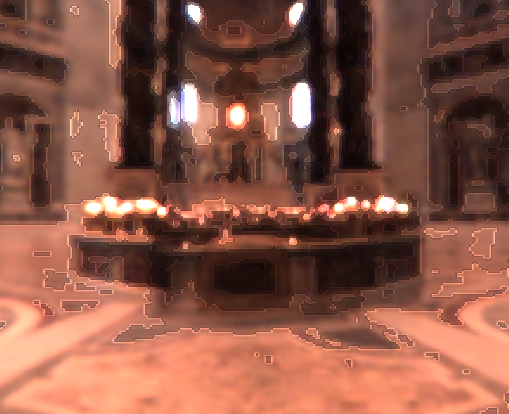
\includegraphics[scale=0.28]{./pics/RGBE_with_GL_RGBA8.png}} 
\subfigure[RGBA12]{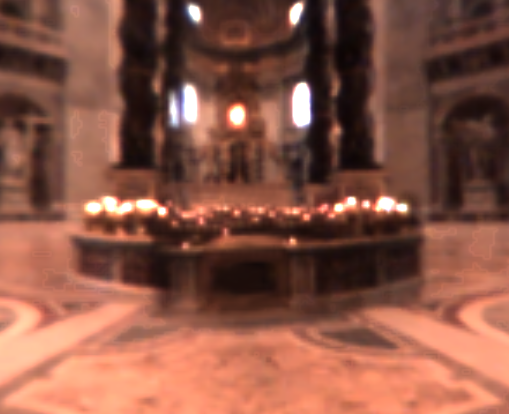
\includegraphics[scale=0.28]{./pics/RGBE_with_GL_RGBA12.png}} 
\subfigure[RGBA16]{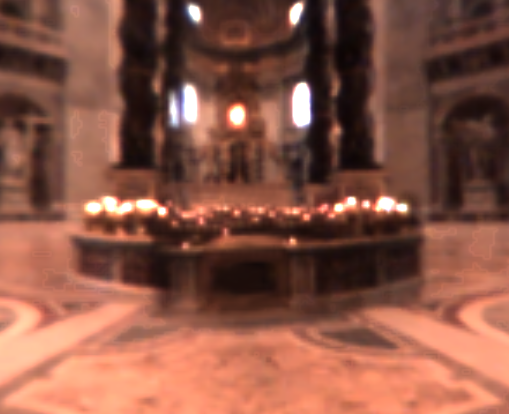
\includegraphics[scale=0.28]{./pics/RGBE_with_GL_RGBA16.png}} 
\caption{Debevec's St. Peters Lightprobe rendered as a cube map. All the scenes are using RGBE decoded values and bilinear filtering.}
\label{fig:RGBEResTest}
\end{figure*}

\subsection{Cube Mapping}
Cube mapping has been used extensively on this project. In order to render the background scene, a vertical cross HDR texture in .hdr format was split into 6 separate .hdr textures (one for each face of the cube). The background scene was then rendered using OpenGL's extension for cube maps. Cube maps were not only used to render the background, but also for IBL. Instead of using a panorama version of the scene, cube maps allow one to fetch the values directly from the cube map texture just by using texture coordinates. Using a panorama image would produce expensive computations on the GPU when converting from a vector representation to the actual texture coordinates. Moreover, it is not necessary to load redundant textures for the same scene - the cube map is used both for IBL and for 
the background rendering.

\begin{figure*}[t]
\centering
{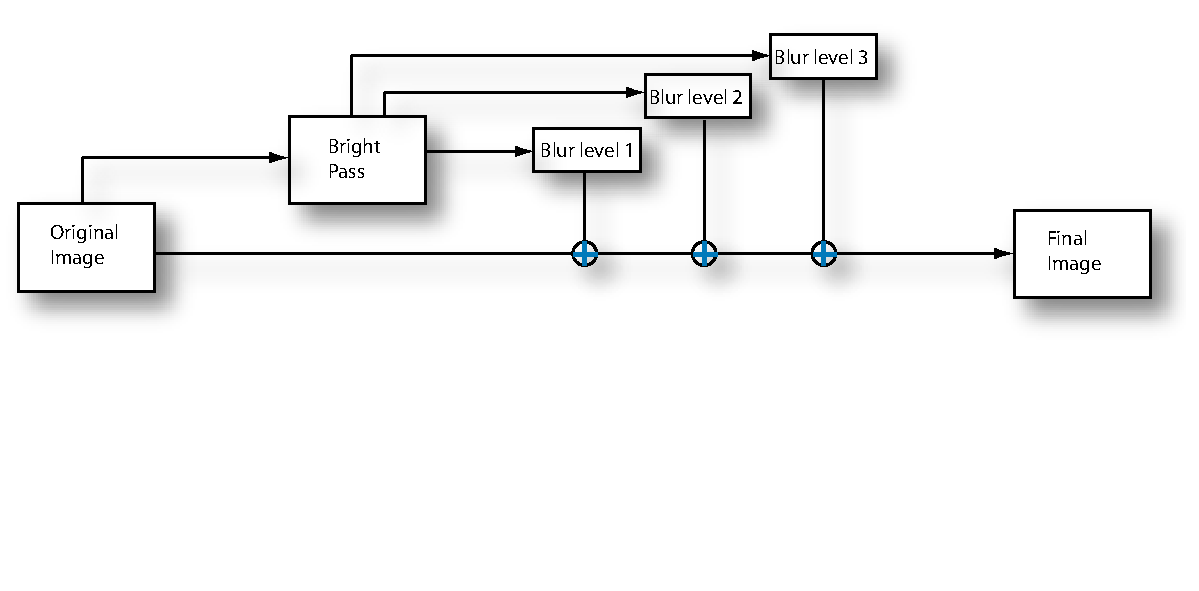
\includegraphics[scale=0.8]{./pics/bloomPipeline.pdf}} 
\caption{Blooming pipeline}
\label{fig:bloomPipeline}
\end{figure*}

\begin{figure*}[t]
\centering
{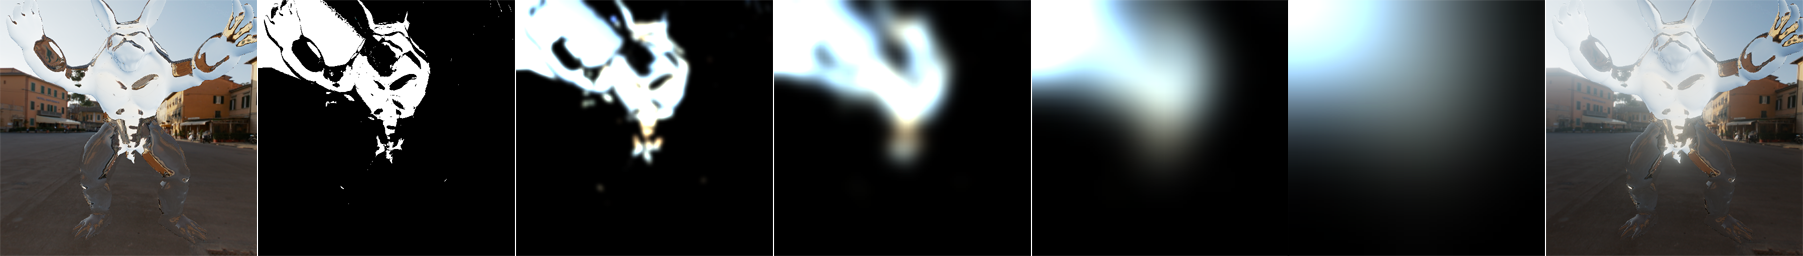
\includegraphics[scale=0.25]{./pics/bloomPipelinePics.png}} 
\caption{Blooming pipeline screenshots}
\label{fig:bloomPipelinePics}
\end{figure*}

\subsection{Tone Mapping}
Tone Mapping is one of the most important parts of this project. Common computer screens do not permit high intensity values to be displayed. However, it is still possible to convey that intensity through that technique (although, it's not exactly the same as showing them as they would be in the real world). Given the scope of the project, real-time issues introduce lots of constraints on what it can and cannot be done while still maintaining interactive frame rates. Therefore, it has been decided to implement a global tone mapping operator instead of a local one (it is possible to do it, however, with some loss on FPS). Reinhard's photographic tone mapper \cite{reinhardPhoto} can be used as a global tone mapping (fairly reasonable for medium dynamic range images) operator:

\begin{equation}
L(x,y) = \frac{L(x,y)}{L(x,y) + 1}
\end{equation} 

However, it was seen that using luminance values instead of real RGB values for the computations would incur in some loss of color saturation. Therefore, the main compression equation becomes:

\begin{equation}
RGB(x,y) = \frac{RGB(x,y)}{RGB(x,y) + 1}
\end{equation} 

The above presented equation is just the final compression equation. However, auto-exposure for the scene was also desirable. So, the $RGB$ tuple need to be multiplied previously by an exposure coefficient computed on the following way:

\begin{itemize}
\item Compute the key of the scene $\alpha$ using an estimation based on luminance values \cite{reinhardParamEstimation}
\item Calculate the correct exposure $Exp_{correct}$ for the scene dividing $\alpha$ by the scene's log average luminance
\item Compute a $\Delta exposure$ between the correct exposure and an exposure gotten from a scene half second before - base exposure.
\item Compute the current exposure $Exp_{current}$ by using the previous exposure $Exp_{prev}$, the delta and a ratio (0.1 in this case) that controls the evolution of the exposure towards the correct one.
\end{itemize}

The base exposure is used so the effect of adaptation is conveyed by using a sort of memory effect of a previous scene.
The previous steps are computed using the following equations:

\begin{equation}
\alpha = 1.2 * 4^{\left(\frac{2\log_2(L_w) - \log_2(L_{min}) - \log_2(L_{max})}{\log_2(L_{max}) - \log_2(L_{min})}\right)}
\end{equation}

\begin{equation}
Exp_{correct} = \frac{\alpha}{\overline{L}_w}
\end{equation}

\begin{equation}
\Delta exposure = \frac{Exp_{correct} + Exp_{base}}{2} - Exp_{prev}
\end{equation}

\begin{equation}
Exp_{current} = Exp_{prev} + \Delta exposure * ratio
\end{equation}

\subsubsection{GPGPU Computations}
Computing luminance statistics for a certain scene might become a heavy operation for real-time applications. Therefore, a General Purpose GPU parallel reduction technique has been used to compute in parallel the minimum, maximum and log average luminance. This technique becomes extremely efficient for scenes bigger or equal to $512^2$ pixels where the parallel power of the GPU comes in. In our particular case the number of pixel pipelines were at least 4 allowing for 4 computations at the same time.

\subsection{Blooming}
Bloom is a graphics effect used to reproduce a human sensation when rapid changes of light intensity occur. The effect produces fringes of light around high intensity light sources and leads to color bleeding on objects near these specific light sources. To be able to obtain a reasonable looking result and a good performance at the same time, a number of optimizations are done.  The blooming pipeline is shown in Figures \ref{fig:bloomPipeline} and \ref{fig:bloomPipelinePics}.

Creating this effect can be described in three main steps. The first step is to apply a high-pass filter which produces a texture that shows the high intensity lights. Applying the high-pass filter (bright-pass) is done by calculating the luminance of the fragment and comparing it to the log average luminance of the original texture. Luminance values higher than the log average luminance will be considered to be of high intensity.

The second step is to apply a radial basis function in the form of a Gaussian kernel to the bright-pass texture to produce a texture that contains the fringes of light. Applying a Gaussian kernel directly to a high resolution texture has a complexity of $O \left ( M \times N \times m \times n  \right )$ where $M \times N$ are the dimensions of the texture being filtered and $m \times n$ are the dimensions of the filter kernel. Thus it shows that applying the kernel in this way is costly and will decrease the performance. 

To keep the performance going and still obtain a good blooming result, adjustments are made to the algorithm. The first change is to linearly separate the Gaussian kernel so it is applied in a vertical and horizontal step. Doing this will change the complexity of the algorithm to $O \left ( M \times N \times m  \right ) + O \left ( M \times N \times n  \right )$ and drastically improve the performance. To be able to linearly separate the Gaussian kernel, a set of Pascal's pyramid is used. On top of this, the two pass technique is applied to different levels of mipmaps of the bright-pass texture. Applying a number of smaller kernel to the low resolution texture gives a close approximation of applying a large kernel to the higher resolution texture. The textures generated at this stage will contain the earlier mentioned fringes and be referred to as blurred textures. When using the RGBE to incorporate HDR information, one should keep in mind that down-sampling and up-sampling using bi-linear filtering might cause the most significant bit of the exponent to toggle (see \cite{hdrTexturing}). The solution to this issue is not to use the RGBE format for this part of the pipeline. Instead 16 bit fixed point textures are used and HDR values going beyond the limit will be clamped to the maximum allowed value.

Once the blurred textures have been created, they are blended with the original image using weights per blur level to form the final bloomed texture. These weights are empirically determined since it is highly affected by the tone mapping. 

\section{Image Based Lighting}

\subsection{Materials}
To show that the environment is lit using image based lighting, four different Bidirectional Reflectance Distribution Functions (BRDF) have been created that are dependant on the lighting environment. The BRDFs implemented are perfect reflection, refraction, diffuse and porcelain. The perfect reflection calculates a reflection vector based on the incident view vector and the normal. This reflection vector is then used to index the cube map which describes the environment. The refraction uses an approximation of the Fresnel equation and calculates the reflectance coefficient at a particular point on the surface. Both the reflection and refraction vector are used to index the cube map and linear interpolation between the fetched texture values is performed using the reflectance to achieve an approximation of a glass-like material. The diffuse material indexes a downsampled diffuse convolution cube map of the environment map using the normal of the object to obtain the appropriate shading. The porcelain material extends on this and uses the Fresnel equation to calculate the amount of specularity the material has on top of the diffuse shading. The approximated Fresnel equation was created by Christophe Schlick and can be found in \cite{opengl-orange-book}.

\subsection{Light probes}
In order to test, build and demonstrate the real-time application, a number of light probes were used to build up the cube maps. The majority of the light probes were taken from Paul Debevec's light probe gallery. On top of this, two self made light probes were also created using a mirror sphere and a digital camera. The mirror sphere was photographed using an aperture of f8.0. The exposure of the camera was set to 1/1000 seconds and the LDR images were taken with 2 f-stops apart. Six light probes are included in the application in the form of cube maps and new environments can be added.

\section{Results}
The obtained results were quite satisfactory and the proposed objective has been achieved. A fully working HDR pipeline has been created using multi-pass shading techniques, IBR and IBL in real-time. The obtained frame rates have exceed the expectations, and the application runs smoothly with 60 fps. It has been proved that all the aforementioned issues can be used in real-time and with the right optimisation more could be added.

\section{Future work}
Future work on this subject could pass by using non-powers-of-two textures (the used ATI cards do not support) with support for MIP Mapping. Floating-point bi-linear filtering would be a good addition in order to discard RGBE encoding and decoding computations. Issues like multisampling and anti-aliasing are also desired features to improve image quality. Finally effects like lens flare, light streaks and chromatic adaptation would also be a plus.

\begin{figure*}[tb]
\centering
\subfigure[Refractive Teapot]{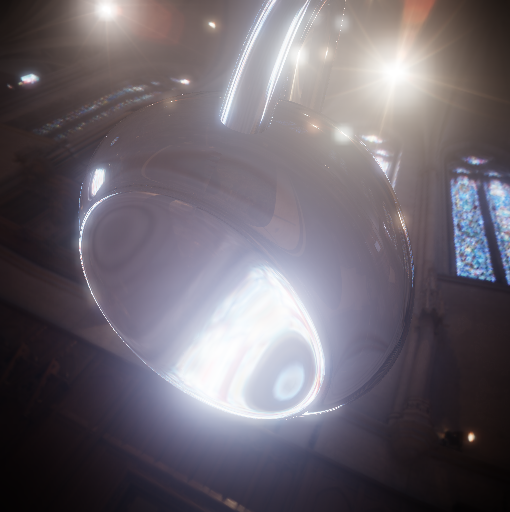
\includegraphics[scale=0.45]{./pics/screenshot1.png}} 
\subfigure[Porcelain Teapot]{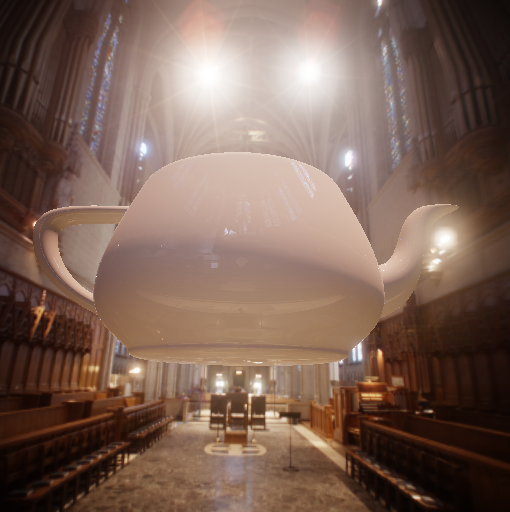
\includegraphics[scale=0.45]{./pics/screenshot2.png}} 
\subfigure[Porcelain Indian Buddha]{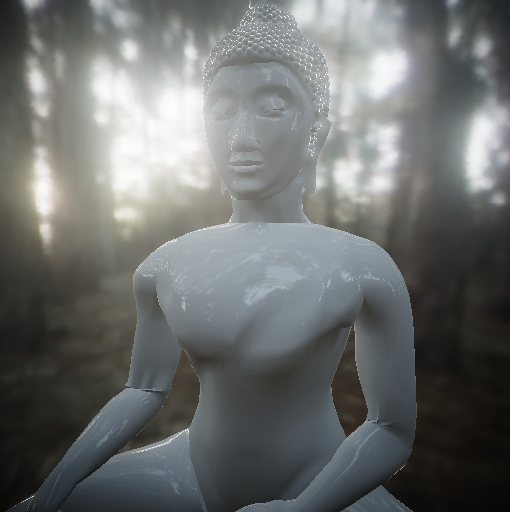
\includegraphics[scale=0.45]{./pics/screenshot3.png}} 
\subfigure[Refractive Double-Headed Dragon]{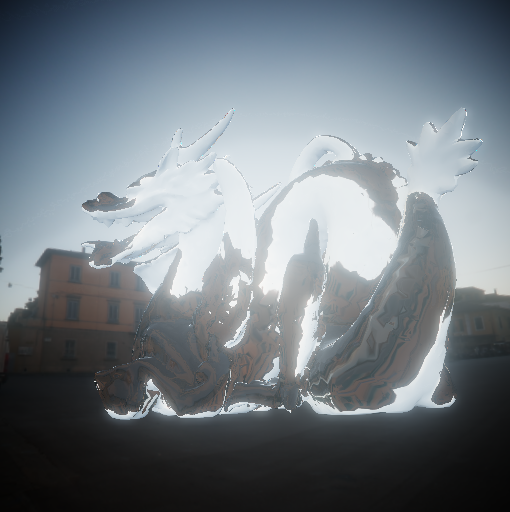
\includegraphics[scale=0.45]{./pics/screenshot4.png}} 
\caption{Screenshots of the application using several materials and light probes.}
\label{fig:screenshots}
\end{figure*}

% ### BIBLIOGRAPHY ###
\bibliography{bibliography}{}
	\bibliographystyle{plain}
\end{document}
